%% INTRO %%
Consider the deformable model of a liver shown in the left of Figure~\ref{fig:liver-multimodel}.
It is surrounded by different anatomical structures (including the diaphragm, the ribs, the stomach, the intestines...) and is also in contact with a grasper (modeled as an articulated rigid chain).
In SOFA, this liver is simulated using three different representations: the first is used to model its internal mechanical behavior, which may be computed using Finite Element Method (FEM) or other models.
The geometry of the mechanical model is optimized for the internal force computations, e.g. one will try to use a reduced number of well-shaped tetrahedra for speed and stability.
However, we may want to use different geometrical models for visualization or contact computation.
The second representation is used for collision detection and response, while the third is dedicated to the visual rendering process.
This sections presents these representations and their connections.

\begin{figure}
 \centering
 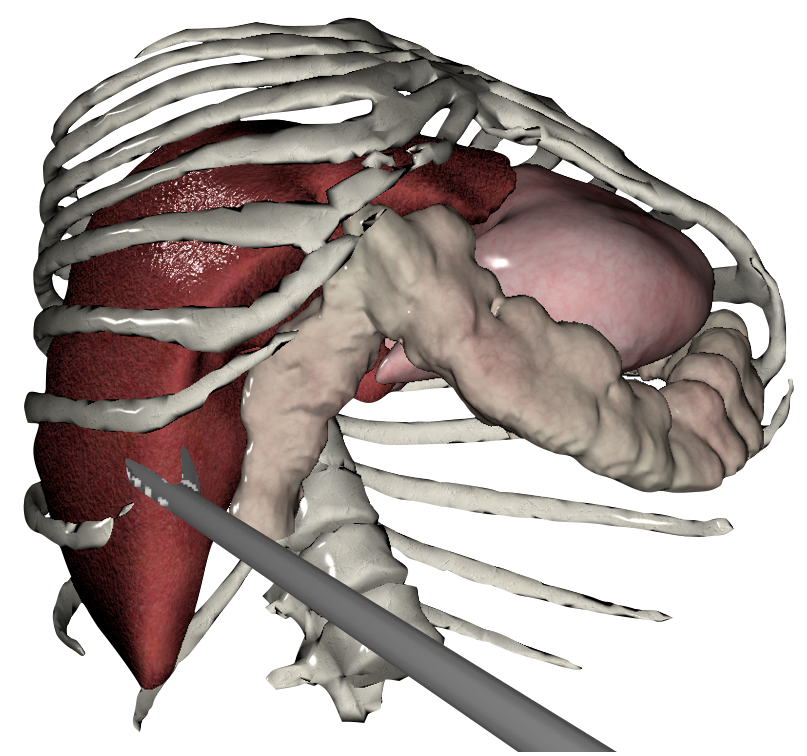
\includegraphics[width=0.48\linewidth]{NewLiver.png}
 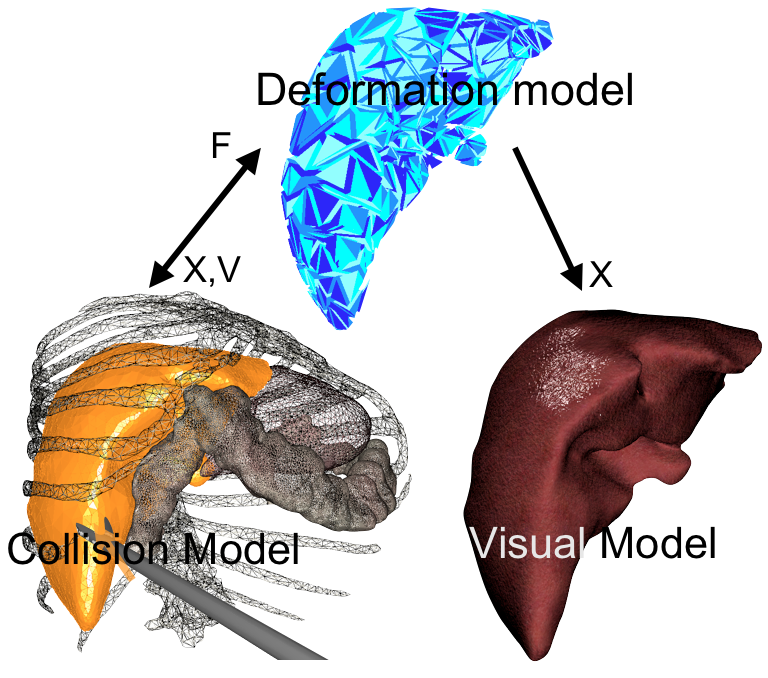
\includegraphics[width=0.5\linewidth]{NewLiverMap.png}
 \caption{A simulated Liver
Left: The simulation of the liver (dataset from IRCAD, France). Right: Three representations are used for the liver: one for the internal mechanics, one for the collisions, and one for the visualization.  These representations are linked using mappings (black arrows).}
 \label{fig:liver-multimodel}
\end{figure}

\section{Solid Mechanics} \label{sec:rigidAndDeformable}


Different models can be employed to discretize a deformable solid continuum as a dynamic or quasi-static system of particles (also called simulation nodes).
The node coordinates are the independent degrees of freedom (DOFs) of the object, and they are typically governed by equations of the following type:
% Some boundary conditions, composed of imposed motion at the node can be applied to the system.
\begin{equation}
 \label{eq:expliciteulerexample}
 \Va = \P \M^{-1} \sum_i \Vf_i (\Vx,\Vv)
\end{equation}
where \Vx and \Vv are the position and velocity vectors, the $\Vf_i$ are the different force functions (volume, surface and external forces in this example), \M is the mass matrix and \P is a projection matrix to  enforce boundary conditions on displacements. Note that the modeling of rigid body dynamics leads to the same type of equations.

The corresponding model in \sofa{} is a set of components connected to a common graph node, as shown in the right of Figure~\ref{fig:liver-mechanical}. 
%
\begin{figure}
 \centering
 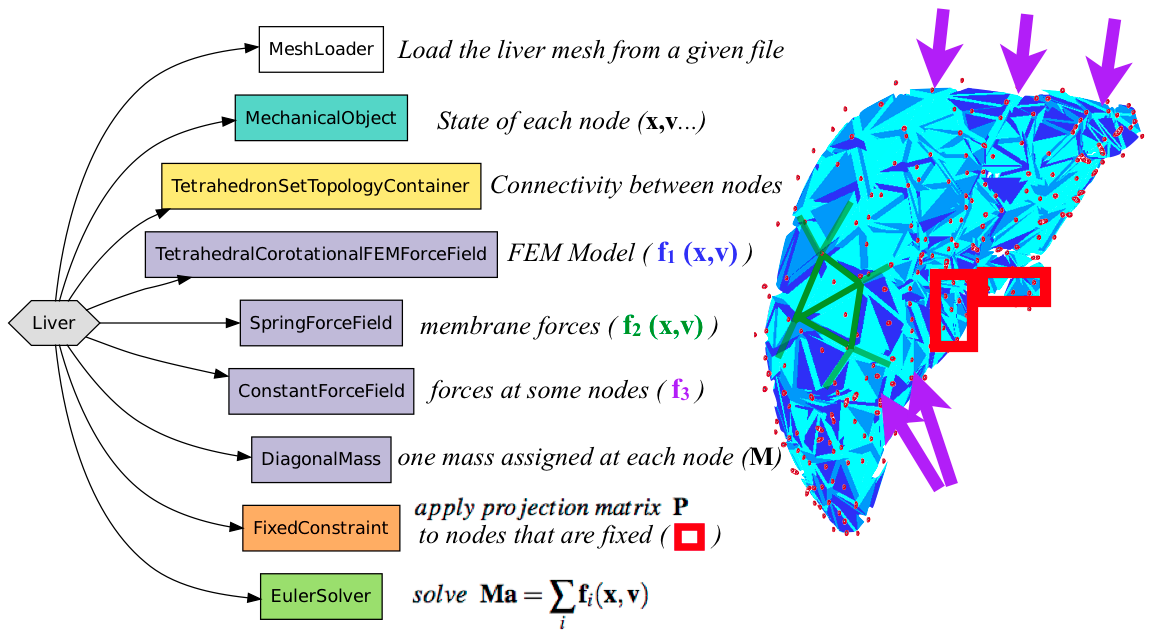
\includegraphics[width=0.95\linewidth]{liver-mechanical2.png}   % generated from ps using: dvipdf -dEPSCrop
 \caption{Mechanical model of a liver. In order to facilitate the combination of models and algorithms, the liver is described as a composition of specialized components.}
 \label{fig:liver-mechanical}
\end{figure}
%
Each component is responsible for a small number of tasks implemented using virtual functions in an object-oriented approach.
Each operator in Equation~\ref{eq:expliciteulerexample} corresponds to a component.
\textit{MeshLoader} is used to read the topology and the geometry.
The coordinate vector \Vx of the mesh nodes and all the other state vectors (velocity \Vv, net force $\sum \Vf$, etc.) are stored in \textit{MechanicalObject}, which is the core component of the mechanical model.
A tetrahedral connectivity is stored in \textit{TetrahedronSetTopologyContainer}, and made available to other components such as \textit{TetrahedralCorotationalFEMForceField}, which accumulates one of the terms of the force sum using the Finite Element method.
The two other terms come from \textit{SpringForceField}, which accumulates the forces generated by the membrane, and  \textit{ConstantForceField}, which accumulates external forces to a given subset of simulation nodes (for instance the pressure exerted by the diaphragm on the liver).
\textit{DiagonalMass} is used to implement the product with matrix $\M^{-1}$.
\textit{FixedConstraint} implements the product with matrix $\P$ to cancel the displacements of the squared particles.
\textit{EulerSolver} implements the logic of time integration.

This approach is highly modular because the components are completely independent of each other and are implemented using C++ classes with a reduced number of abstract functions. 
For instance, in the example of figure \ref{fig:liver-mechanical}, if one want to use a FEM for the membrane force instead of the spring based computation, only \textit{SpringForceField} has to be changed for \textit{TriangleFEMForceField}. Similarly, the mass matrix, stored as diagonal matrix in this example, can be stored as a single scalar value (\textit{UniformMass}) if less accuracy but faster computation is sought, in combination with an iterative solver for instance.



For efficiency, each mechanical state vector contains the values of all the simulation nodes, to avoid multiple call of virtual function resolutions.
The vector size is basically the number of particles times the number of space dimensions. 
We use C++ templates to avoid code redundancy between scalar types (float, double), the types of degrees of freedom (particles, frames, generalized coordinates), and the number of space dimensions.
All the particles in a vector have the same type known at compile time.
Degrees of freedom of different types must be grouped in different objects, possibly connected with interaction forces, as discussed in Section~\ref{sec:interactionforcefield}.
This greatly simplifies the design and allows aggressive compiler optimizations.

More than 30 classes of forces are implemented in SOFA, including springs, FEM for volumetric (tetrahedron or hexahedron) or surface (triangular shell and membrane) deformable objects using corotational or hyperelastic formulations, and for wire or tubular object (beam models meshed with segments), have been implemented.
Different types of springs allow for easy and fast modeling of the deformations (bending, compression/traction, volume, interactions between two bodies, joints...).
In rigid objects, the main components are the degrees of freedom (a single frame with 3 rotations and 3 translations) and the mass matrix that contains the inertia of the object. 
Surfaces can be attached to objects using \textit{mappings}, as discussed in Section~\ref{sec:mappings}.


\section{Collision models} \label{sec:collisionModels}
When a lot of primitives comes into contact, collision detection and response can become the bottleneck of a simulation. 
Several collision detection approaches have been implemented: distances between pairs of geometric primitives (triangles and spheres), points in distance fields, distances between colliding meshes using ray-tracing~\cite{HerFauRaf08}, and intersection volume using images~\cite{AFCFDK10}
The collision pipeline is described in section \ref{sec:collision} with more details. 

In order to adapt the models to the data structure of the different collision algorithms, we have defined a \textit{collision model}.
This model is similar to a mechanical model, except that its topology and its geometry are of its own and can be  stored in a data structure dedicated to collision detection. 
For instance, the component \textit{TriangleModel} is the interface for the computation of collision detection on a triangular mesh surfaces.

If the collision of a given simulation takes too much time, or to reduce the number of collision points, the meshes used for collision detection can be chosen less detailed than the mechanical ones. 
In the opposite, if precise collision detection and response is needed with  smooth surfaces, it is sometimes suitable to use more detailed mesh for collision detection.











%%%%%%%%%%%%%%%%%%%%%%%%%%%%%%%
\section{Visual models} \label{sec:visual}

In the context of surgical simulation for training, to reach the state of what is often called \textit{suspension of disbelief} i.e. when the user forgets that he or she is dealing with a simulator, there are other factors than the mechanical behavior. 
Realistic rendering is one of them. 
It involves visually recreating the operating field with as much detail as possible, as well as reproducing visual effects such as bleeding, smoke, lens deformation, etc.
The main feature of the visual model of SOFA is that the meshes used for the visualization can be disconnected from the models used for the simulation. 
The mappings described in section \ref{sec:mappings} maintain the coherency between them.
Hence, SOFA simulation results can easily be displayed using models much more detailed than used for internal mechanics, and rendered using external libraries such as OGRE\footnote{www.ogre3d.org} and Open Scene Graph\footnote{www.openscenegraph.org}.

We have also implemented our own rendering library based on openGL. 
This library allows for modeling and render the visual effects that occurs during an intervention or the images that the surgeon is watching during the procedure.
For instance, in the context of interventional radiology simulator, we have developed  a dedicated interactive rendering of X-ray and fluoroscopic images. 




